%!TEX root = ../thesis.tex
%*******************************************************************************
%*********************************** Nineth Chapter *****************************
%*******************************************************************************

\chapter{Comparison between iPG measurements and other sensors}  %Title of the First Chapter

\ifpdf
\graphicspath{{Chapter9/Figs/Raster/}{Chapter9/Figs/PDF/}{Chapter9/Figs/}}
\else
\graphicspath{{Chapter9/Figs/Vector/}{Chapter9/Figs/}}
\fi


%%********************************** % Section 9.1 ******************************************
\section{Measurements from the ECG device}
\label{section comparison 4}
The ECG signals collected provide details of the electrical activity of the heart during the whole study. Hence, no changes were registered through the test unless a bad connection occurred. The data gathered works as a clock reference during the data processing. Additionally, it helped as a reference to calculate pulse transit time with the other dynamic signals obtained. \mynote{Check if I am going to publish measurements about PTT. If not this paragraph should be modified}. Figure \ref{fig:ECG} shows the typical ECG for one of the participants.

\begin{figure}[!htbp]
	\centering
	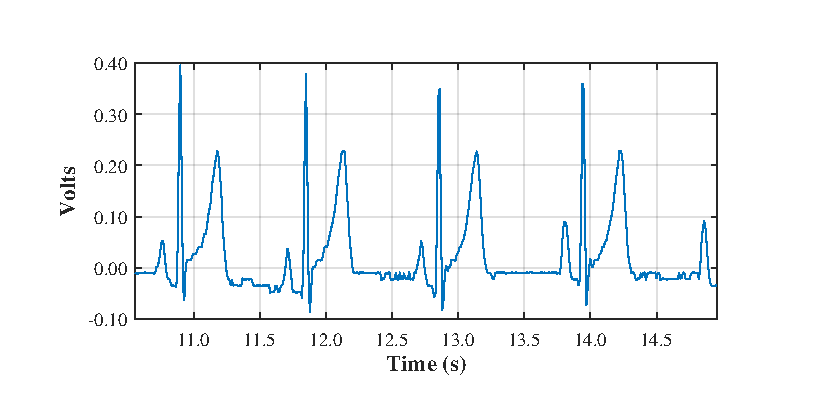
\includegraphics{figure19}    
	\caption[ECG measurement acquired by the system]{Measurement from one of the participants. Clearly, it can be identified the points P, Q, R, S and T. This signal did not change during the whole experiment.}
	\label{fig:ECG}
\end{figure} 

All the waveforms detected were normal and provided enough information about the characteristic peaks in an ECG waveform. The points P, Q, R, S and T are clearly visible in all the signals. Nonetheless, participant 1 showed an elevated T wave which is presumably due to his athletic career. According to him, he had a ventricular hypertrophy meaning that one of his ventricles was enlarged.  

%%********************************** % Section 9.2 ******************************************
\section{Blood flow estimation from Doppler ultrasound instrument}
\label{section comparison 1}
As part of the experimental procedure, a Doppler ultrasound was used to estimate blood flow using the radial artery in the wrist as a reference. The raw data produced by the instrument came in volts and were converted into more meaningful data using the equations \ref {eq:doppler} and \ref {eq:flow_l/min} which convert the information into units\nknote{do you need to say units here?} litres per minute (\si{\litre\per\minute}). As described in those equations, the angle was set at \SI{45}{\degree} using a laboratory support and a clamp. The cross-sectional area for calculating blood flow was the median value of~\cite {ashraf2010size}. The head of the ultrasound device was placed as close to the artery as described in the user manual of the instrument using a conductive gel.

While taking the measurements, there was an electrical problem with the Doppler ultrasound instrument. Hence, it was not possible to collect data from participant 8. The data presented in \ref{fig:DU_flow} and \ref{tbl:DU flow} contains the results of the first seven participants.

\begin{figure}[!htb]
	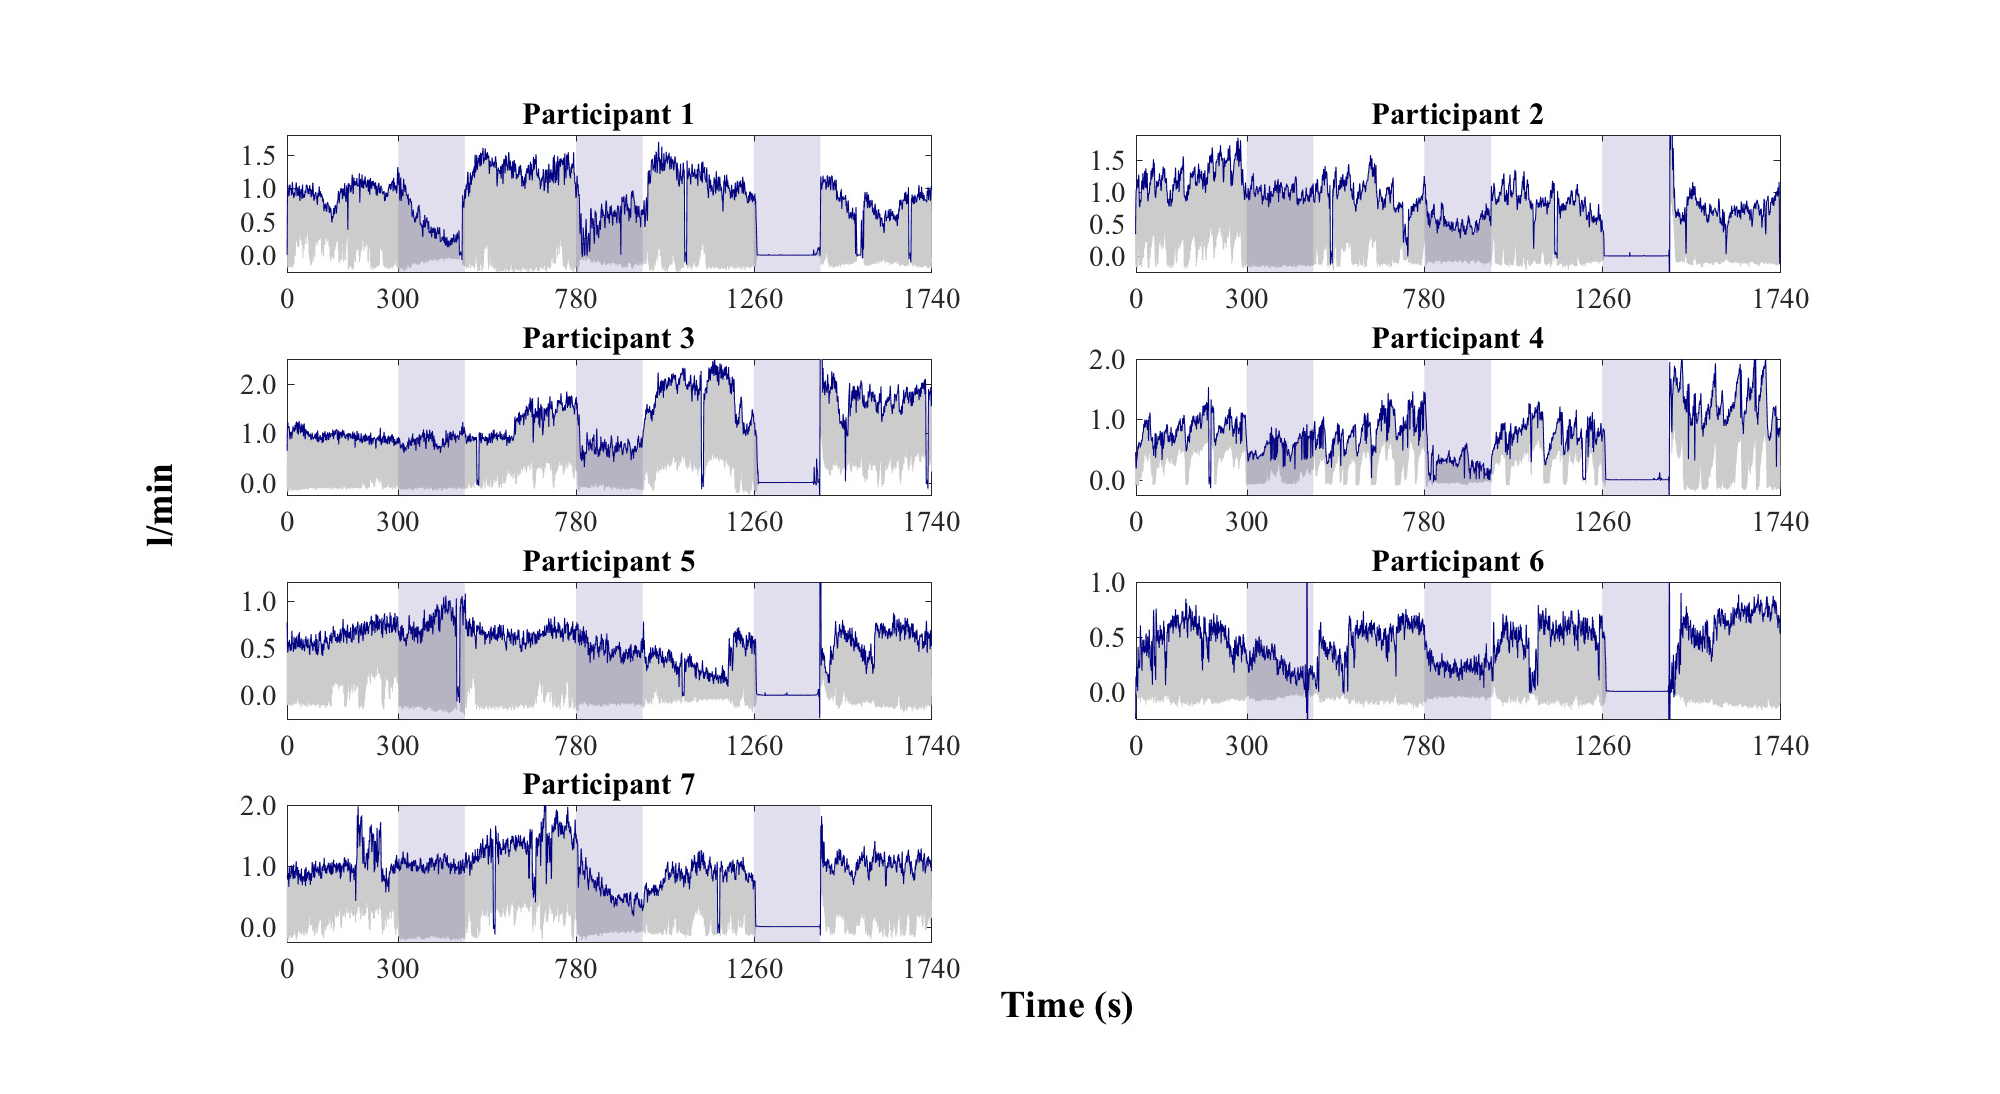
\includegraphics[width=\textwidth,height=\textheight,keepaspectratio,trim={2.5cm 0cm 2.5cm 0 cm},clip]{figure16}    
	\caption[Blood flow calculated from Doppler ultrasond device all along the whole expetiment]{Blood flow calculated from the Doppler ultrasound measurements for all the participants during the experiment. The greyed out areas are the raw sign of the DU waveform. The dark blue lines represent the envelope calculated from the peak values. The blood flow was converted to the units (\si[per-mode=symbol]{\litre\per\minute}).}
	\label{fig:DU flow}
\end{figure}

Figure \ref{fig:DU flow} shows the peak values of the Doppler ultrasound converted into the blood flow. The shaded areas represent the occlusive events during the study. From a quantitative point of view, evidently, various participants showed a decline in their flow during venous occlusion in region 2.  Participant 1 evidenced an exponential flow rate decrease during this part of the test. Moreover, participants 2 and 4 displayed a quick drop within the first seconds followed by a levelling at a mid-point. On the other hand, the rest of the participants did not show a significant change in flow rate during this transition. When the cuff's pressure was released only participants, 1 and 6 showed blood flow returning to the baseline value.  

During partial arterial occlusion, the change of arterial blood flow is unmistakable in most of the participants. Only, participant 5 did not register a large shift in the circulatory flow. In contrast, all the \nknote{?the word other may be needed here? }participants showed a lack of signal during total occlusion. 

The numbers of the mean blood flow rate described in table \ref{tbl:DU flow} are different from the ones shown in the figure. In general, in the transition from baseline to venous occlusion, most of the participants experienced a drop of blood flow. The decline of the blood flow in region 2 was on average \SI{0.261(0134)}{\litre\per\min}. In contrast, participants 5 and 7 experienced a slight increase in the flow rate of approximately -0.055(0.062) l/min. After releasing the cuff's pressure, most participants showed an increase in their measured flow rate of about \SI{0.386(0231)}{\litre\per\min}. Participants 2 and  5 showed a decrease in their flow of \SIlist{-0.049;-0.084}{\litre\per\min}. 

\begin{table}[!htbp]
	\caption{Mean blood flow calculated form the plethysmography wave for baseline, total occlusion and return to normality}
	\label{tbl:DU_flow}
	\centering \small
	\begin{tabular}{lcccccccc}
		\toprule
		& \textbf{Region 1}
		& \textbf{Region 2}
		& \textbf{Region 3}
		& \textbf{Region 4}
		& \textbf{Region 5}
		& \textbf{Region 6}
		& \textbf{Region 7} \\
		& \textbf{[\si[per-mode=symbol]{\litre\per\minute}]}
		& \textbf{[\si[per-mode=symbol]{\litre\per\minute}]}
		& \textbf{[\si[per-mode=symbol]{\litre\per\minute}]}
		& \textbf{[\si[per-mode=symbol]{\litre\per\minute}]}
		& \textbf{[\si[per-mode=symbol]{\litre\per\minute}]}
		& \textbf{[\si[per-mode=symbol]{\litre\per\minute}]}
		& \textbf{[\si[per-mode=symbol]{\litre\per\minute}]} \\\midrule
		Participant 1    &     0.944     &     0.486     &     1.278     &     0.583     &     1.110     &     0.041     &     0.731     \\  
		Participant 2    &     1.245     &     1.003     &     0.954     &     0.551     &     0.841     &     0.013     &     0.760     \\  
		Participant 3    &     0.942     &     0.859     &     1.190     &     0.747     &     1.797     &     0.082     &     1.681     \\  
		Participant 4    &     0.823     &     0.543     &     0.817     &     0.305     &     0.755     &     0.040     &     1.266     \\  
		Participant 5    &     0.639     &     0.737     &     0.654     &     0.502     &     0.362     &     0.036     &     0.589     \\  
		Participant 6    &     0.496     &     0.256     &     0.477     &     0.240     &     0.499     &     0.029     &     0.600     \\  
		Participant 7    &     1.009     &     1.021     &     1.330     &     0.622     &     0.841     &     0.021     &     1.044     \\  
		\bottomrule
	\end{tabular}
\end{table}

During partial arterial occlusion, all the participants showed a decrease in their blood flow rate. On average, there was a reduction of \SI{-0.449(0212)}{\litre\per\min}. Which\nknote{??whihc wrong word what do you mean} data is entirely in agreement with the partial restriction of their arterial blood flow. However, when the blood flow was restored from region 4 to 5 most of the partakers showed an increase in their blood flow. The increment of blood flow was on average \SI{0.466(0310)}{\litre\per\min}. The only one registering a decrease in the median was participant 5 which dropped \SI{0.141}{\litre\per\min}. 

During total occlusion, all the participants showed an extreme decrease in their measured circulatory flow rate. As expected, no arterial or venous flow was recorded, the registered values might represent artefacts in the signals. After releasing the tourniquet, all the participants experienced an increase in their flow rate to values of normality. 

%%********************************** % Section 9.3 ******************************************
\section{Measurements from Laser Doppler Flowmetry}
\label{section comparison 2}
The LDF device provided raw data in Volts which was converted into BPU units. This conversion was possible by applying equation \ref{eq:BPU} to the data collected.  As explained in section \ref{section:ldf}, the result produced is in arbitrary units which represent blood cell movement under the skin. Therefore, it illustrates the blood flow moving red blood cells in the micro-circulatory bed to distal parts of the tissue in the forearm.

Figure \ref{fig:LDF flow} displays the peaks of the LDF waveform signal in BPU. A moving average was used to aggregate 20 seconds of data to the resultant plot. That plot shows that the movement of the cell is affected when an occlusion occurs. It must be noted that a noise artefact heavily impacted some parts of the data. Such as in participants 1 and 4.

\begin{figure}[!htb]
	\centering
	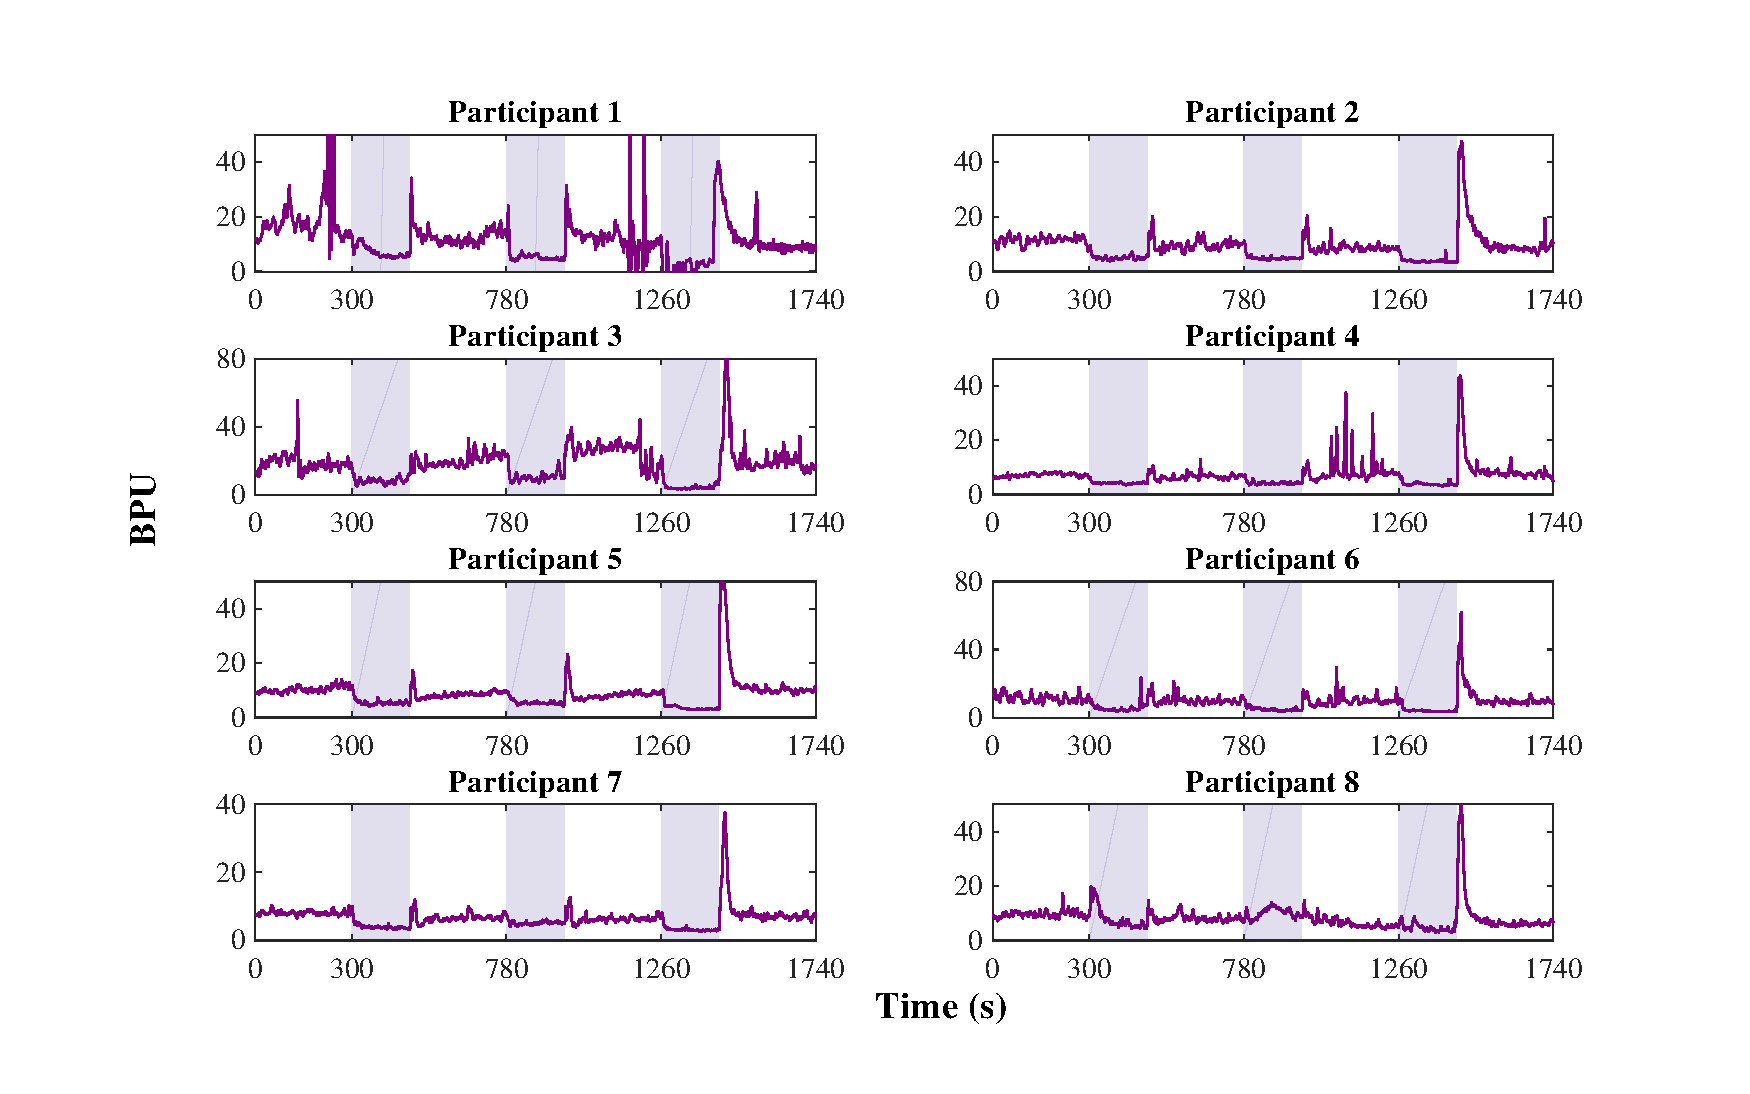
\includegraphics[width=\textwidth,height=\textheight,keepaspectratio,trim={2cm 0cm 2cm 0 cm},clip]{figure17}    
	\caption[Results of the LDF in BPU]{Results of the Laser Doppler Flowmetry measurement for all the participants after being converted to BPU. The values presented in purple are equivalent to envelope signal of the peak points.}
	\label{fig:LDF flow}
\end{figure}

Nevertheless, a trend can be noticed in all the participants. During the occlusion in region 2, a slight decline in cell movement can be noticed. It shows that the venous occlusion slowed down the movement of RBC. After the cuff's pressure was released, a peak can be seen in most of the participants. This hyperaemic effect shows an acceleration of the RBC after the blockage event. 

Similar effects can be seen during partial arterial occlusion; the cells speed reduced compared to the previous baseline (region 3). Then as soon as the blockage was released, again the rush of RBCs can be detailed. Nevertheless, participant 8 seems to be an exception to the rule. His BPU tends\nknote{not sure if tends is good here} to increase slightly during the transition of region 3 to 4. Moreover, contrary to the other signals in the transition from partial arterial occlusion to baseline in region 5, his BPU decreased. These results also could explain some of the adverse readings captured by the iPG signals.

Lastly, during total occlusion, all the mean BPUs of the participants reduced considerably. Then later, when the tourniquet was released, the rush of blood flow can be noticed in the hyperaemic effect registered by the instrument, which was also detected by others instruments.

Table \ref{tbl:LDF flow} reviews the values of the mean BPU data obtained. The results declared there, are in complete agreement with the figure previously analysed.

\begin{table}[!htbp]
	\caption{Mean blood flow calculated form the plethysmography wave for baseline, total occlusion and return to normality}
	\label{tbl:LDF flow}
	\centering \small
	\begin{tabular}{lcccccccc}
		\toprule
		& \textbf{Region 1}
		& \textbf{Region 2}
		& \textbf{Region 3}
		& \textbf{Region 4}
		& \textbf{Region 5}
		& \textbf{Region 6}
		& \textbf{Region 7} \\
		& \textbf{[BPU]}
		& \textbf{[BPU]}
		& \textbf{[BPU]}		
		& \textbf{[BPU]}		
		& \textbf{[BPU]}
		& \textbf{[BPU]}
		& \textbf{[BPU]}\\\midrule
		Participant 1    &     42.89     &     12.71     &     18.37     &      9.52     &     36.44     &     11.75     &     19.64     \\  
		Participant 2    &     17.05     &      9.18     &     15.24     &      8.32     &     14.38     &      6.46     &     21.22     \\  
		Participant 3    &     30.69     &     17.08     &     33.42     &     20.72     &     40.28     &      9.27     &     38.08     \\  
		Participant 4    &     10.14     &      6.27     &     10.61     &      7.18     &     16.22     &      6.67     &     15.73     \\  
		Participant 5    &     16.66     &     10.49     &     14.16     &      9.56     &     14.58     &      5.73     &     23.70     \\  
		Participant 6    &     19.82     &     11.41     &     18.43     &      9.75     &     17.87     &      7.83     &     19.14     \\  
		Participant 7    &     12.54     &      7.45     &     11.08     &      9.32     &     10.96     &      5.91     &     14.83     \\  
		Participant 8    &     15.76     &     13.54     &     14.36     &     17.74     &     12.33     &      9.21     &     16.08     \\  
		\bottomrule
	\end{tabular}
\end{table}


%%********************************** % Section 9.4 ******************************************
\section{Measurements Red-light from PPG signal}
\label{section comparison 3}
The PPG device provides information about the change of volume within the vascular bed under the skin. It is capable of detecting either venous or arterial blood change according to the light wavelength being used \mynote{check if this is true or find a reference}. The device employed in the experiment has an output port which provides the unprocessed raw photoplethysmography waveform. Similarly, as in the iPG signal, the PPG is composed of DC and AC parts. The DC portion of the signal is equivalent to the blood volume under the light beam. It also contains data about respiratory rate and other physiological information. On the other hand \nknote{not good use of on the other hand}, the AC component changes in amplitude synchronously according to the cardiac cycle and blood volume in the capillaries. 

During the experiment performed changes in DC and AC components can be easily identified \nknote{doesnt make sense} as showed in figure \ref{fig:RED PPG}. In the plot, the shaded regions represent each occlusive event during the test. On the left, the DC component of the PPG per participant is illustrated. This signal was obtained by detecting the low envelope values of the raw PPG waveform. In other words, the points on the foot of the waveform.  On the right-hand side is the AC component of the signal obtained by removing the low envelope of the raw data. Next, the waveform was inverted to leave only the dynamic element of the signal. Last, the peaks detected from the plethysmography waveform were redrawn in black, highlighting the maximum values during all the occlusive events.  

\begin{figure}[!htbp]
	\centering
	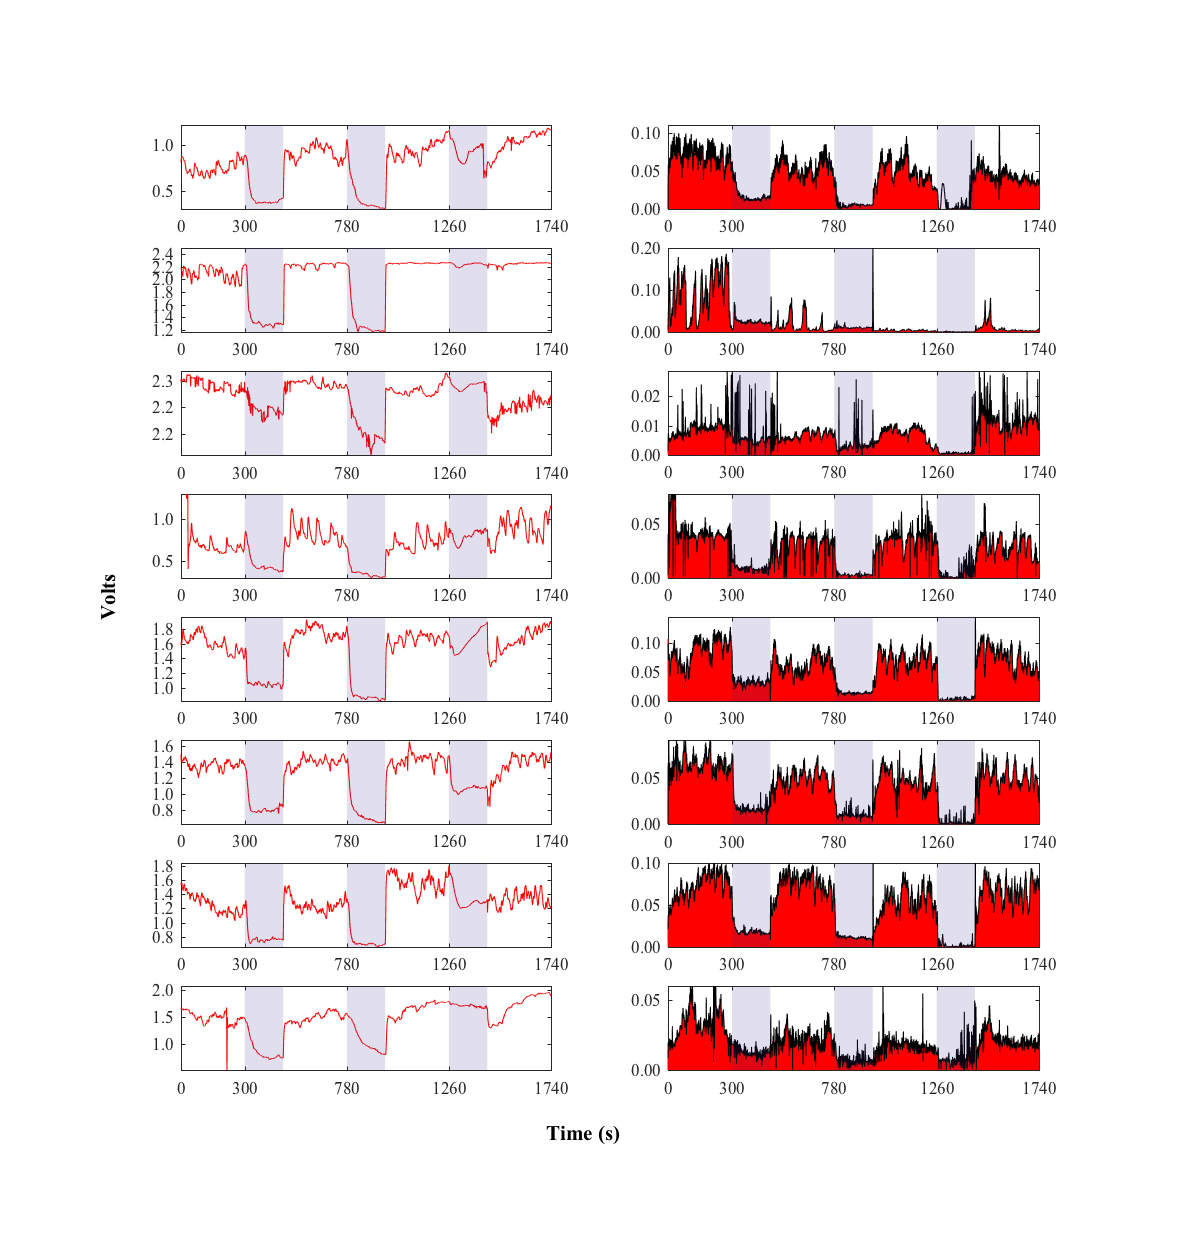
\includegraphics[width=\textwidth,keepaspectratio,trim={1cm 0cm 0cm 0 cm},clip]{figure18}    
	\caption[PPG red wavelength measurments AC and DC components]{Measurements from the red wavelength PPG sensor. On the left, the DC component of the signal, ?? it only includes the lower envelope of the waveform. On the right, the AC component of the red wavelength where the foot of the signal has been aligned to zero ??. The envelope showed in black describes the peaks of the signal}
	\label{fig:RED PPG}
\end{figure}
\nknote{??}

\begin{table}[!htbp]
	\caption[Mean peak value of the PPG DC signal for all participants in all regions]{Mean peak value of the PPG DC signal for all the participants in all the regions.}
	\label{tbl:PPG RED DC}
	\centering \small
	\begin{tabular}{lcccccccc}
		\toprule
		& \textbf{Region 1}
		& \textbf{Region 2}
		& \textbf{Region 3}
		& \textbf{Region 4}
		& \textbf{Region 5}
		& \textbf{Region 6}
		& \textbf{Region 7} \\
		& \textbf{[\si{\volt}]}
		& \textbf{[\si{\volt}]}
		& \textbf{[\si{\volt}]}		
		& \textbf{[\si{\volt}]}		
		& \textbf{[\si{\volt}]}
		& \textbf{[\si{\volt}]}
		& \textbf{[\si{\volt}]}\\\midrule
		Participant 1    &     0.75      &     0.44      &     0.91      &     0.43      &     0.94      &     0.91      &     1.03      \\  
		Participant 2    &     2.09      &     1.38      &     2.22      &     1.33      &     2.25      &     2.24      &     2.24      \\  
		Participant 3    &     2.24      &     2.20      &     2.24      &     2.16      &     2.23      &     2.24      &     2.20      \\  
		Participant 4    &     0.76      &     0.46      &     0.80      &     0.36      &     0.72      &     0.79      &     0.89      \\  
		Participant 5    &     1.60      &     1.07      &     1.73      &     0.93      &     1.66      &     1.64      &     1.64      \\  
		Participant 6    &     1.36      &     0.84      &     1.38      &     0.76      &     1.41      &     1.08      &     1.35      \\  
		Participant 7    &     1.26      &     0.79      &     1.25      &     0.75      &     1.56      &     1.32      &     1.34      \\  
		Participant 8    &     1.48      &     0.88      &     1.48      &     1.07      &     1.64      &     1.71      &     1.70      \\  
		\bottomrule
	\end{tabular}
\end{table}

From the DC signal point of view, all the participants showed a clear drop in their DC components of the signal during venous occlusion (region 2) and partial arterial occlusion (region 4). The figure clearly portrays, that the DC value dropped dramatically in most participants after the occlusive event. Nevertheless, participant 3 showed an exponential decrease in his recorded readings. Effectively, these changes can be clearly confirmed when analysing the mean values of the DC data described in Table \ref{tbl:PPG RED DC}. From there, it is calculated that the average baseline before the occlusions were \SI{1.44(055)}{\volt} for Region 1 and \SI{1.51(054)}{\volt} for Region 3. During the occlusive transitions, the DC components dropped about \SI{-0.435(0210)}{\milli\volt} and \SI{-0.528(0247)}{\milli\volt} for region 2 and region 4 respectively. Nevertheless, during total occlusion, the signals obtained were erratic with no clear shape or direction. Some participants showed a slight decrease, but others did not exhibit significant changes. In general, DC data provided valuable information during the venous and partial arterial occlusion but not conclusive results during total blood flow stoppage. 

\begin{table}[!htbp]
	\caption[Mean peak value of the PPG AC signal for all participants in all regions]{Mean peak value of the PPG AC signal for all the participants in all the regions.}
	\label{tbl:PPG RED AC}
	\centering \small
	\begin{tabular}{lcccccccc}
		\toprule
		& \textbf{Region 1}
		& \textbf{Region 2}
		& \textbf{Region 3}
		& \textbf{Region 4}
		& \textbf{Region 5}
		& \textbf{Region 6}
		& \textbf{Region 7} \\
		& \textbf{[\si{\milli\volt}]}
		& \textbf{[\si{\milli\volt}]}
		& \textbf{[\si{\milli\volt}]}		
		& \textbf{[\si{\milli\volt}]}		
		& \textbf{[\si{\milli\volt}]}
		& \textbf{[\si{\milli\volt}]}
		& \textbf{[\si{\milli\volt}]}\\\midrule
		Participant 1    &     724.83    &     180.45    &     546.76    &      66.13    &     490.87    &     109.85    &     441.54    \\  
		Participant 2    &     926.02    &     245.24    &     158.34    &     110.32    &      51.30    &       5.97    &      92.58    \\  
		Participant 3    &      94.21    &      69.72    &      68.76    &      37.19    &      71.62    &      10.54    &     122.67    \\  
		Participant 4    &     436.74    &      92.42    &     315.26    &      37.22    &     354.44    &      58.08    &     296.36    \\  
		Participant 5    &     873.38    &     324.60    &     638.53    &     155.21    &     703.81    &      51.36    &     751.62    \\  
		Participant 6    &     658.05    &     188.75    &     501.10    &     112.57    &     480.41    &      38.14    &     517.01    \\  
		Participant 7    &     731.50    &     190.43    &     746.34    &     125.76    &     547.89    &      26.92    &     660.43    \\  
		Participant 8    &     360.69    &     130.06    &     216.80    &      74.43    &     168.52    &      89.77    &     217.06    \\ 
		\bottomrule
	\end{tabular}
\end{table}

On the other hand \nknote{??use different start}, AC component produced distinctive results during each blockage event. In comparison with the DC, the AC signal was able to detect changes during total occlusion which is concurrent with the fact that there is no change of volume at that moment. Reviewing the AC signals qualitatively, participant 2 registered noisy waveforms during region 1 of the study. In addition, participant 3 had noisy peaks during the whole test, but changes through each occlusion are still visible.

From the numeric point of view, Table \ref{tbl:PPG RED AC} shows the average values of the amplitude in mV. During baseline, the mean peak value was \SI{600.67(28201)}{\milli\volt}, \SI{398.98(24421)}{\milli\volt}, \SI{358.61(23913)}{\milli\volt} and \SI{387.4073(24531)}{\milli\volt} for regions 1,3,5 and 7 respectively. In general, during venous occlusion, the signal amplitude decreased in all participants to about \SI{-422.97(21217)}{\milli\volt}. Participant 5 had the smallest change (\SI{-24.50}{\milli\volt}) compared to the rest of the signals. 

After the cuff's pressure had been released during the transition from venous occlusion to baseline, participants 2 and 3 showed an increase of their mean amplitude. The rest displayed a recovery in their signal peak to a peak of approximately \SI{221.28(21124)}{\milli\volt}. Subsequently, during partial arterial occlusion, all participants showed a decrease in their mean PPG signals amplitude, to an average of \SI{-309.14(21943)}{\milli\volt}. When comparing mean values during occlusions in region 2 and 4, the signal amplitude in region 4 was slightly lower than the one in region 2 by about \SI{-87.86(4691)}{\milli\volt}. 

Finally, during total occlusion, all the participants demonstrated a substantial decrease in their AC amplitudes. All in all, signals went below 109 mv with an average value of \SI{-48.83(3662)}{\milli\volt}.

In conclusion, the PPG waveform experienced changes of DC and AC components during each type of occlusions throughout the study. The DC signal was able to detect changes during venous and partial arterial occlusions. The difference in mean values of these two events was minimal. Nevertheless, the DC component did not show significant changes during total occlusion.  On the other hand, the AC component was able to detect changes during all occlusions. being each mean peak value significantly lowers during each test \nknote{?? improve this sentence}. 


